\chapter{Z Tanım Bölgesinde P Kontrolör Tasarımı}
\begin{enumerate}
    \item Geçici hal yanıtını şekillendirecek isterler dikkate alınarak s tanım bölgesinde baskın kutuplar seçilir. 
    \item Baskın kutuplar $z=e^{sT}$ ilişkisi ile z tanım bölgesine aktarılır. 
    \item Kontrol edilecek sistem Z tanım bölgesine geçirilir. 
    \item Kapalı çevrim transfer fonksiyonu elde edilir ve kutup atama yapılır.
\end{enumerate}
Örnek sistem
\begin{equation}
    G(s)=\frac{1}{s+2}
\end{equation}
z tanım bölgesinde $T=0.2$ olmak üzere
\begin{equation}
    G(z)=\frac{0.1648}{z-0.6703}
\end{equation}
olarak elde edilmektedir. Yerleşme zamanı $t_s=2$ ve aşım $\%10$ isterleri verilmiştir. Bu durumda $\zeta=0.591$ ve $w_n=6.7664$ seçilir. Seçilen sönüm oranı ve doğal frekans ile baskın kutuplar
\begin{equation}
    s_{1,2}=-4 \pm 5.4575i
\end{equation}
şeklinde hesaplanır. $z=e^{sT}$ ifadesi ile z tanım bölgesinde kutuplar
\begin{equation}
    z_{1,2}=0.2072 \pm 0.3987i
\end{equation}
ve kutuplardan oluşturulacak polinom
\begin{equation}
    p(z)=z^2-0.4144 z+0.2019
\end{equation}
olarak hesaplanır. P tipi kontrolör ile kapalı çevrim transfer fonksiyonunun ifadesi
\begin{equation}
\begin{split}
    T(z)&=\frac{kG(z)}{1+kG(z)}\\
    &=\frac{k\frac{0.1648}{z-0.6703}}{1+k\frac{0.1648}{z-0.6703}}\\
    &=\frac{k(0.1648)}{z-0.6703+k(0.1648)}\\
    &=\frac{0.1648k}{z+0.1648k-0.6703}
\end{split}
\end{equation}
şeklindedir. Görüldüğü üzere karakteristik polinom birinci dereceden elde edilmiştir ve her iki isterlerin sağlanması mümkün değildir. Yerleşme zamanı sağlanmak istenirse,
\begin{equation}
    s=-\frac{4}{t_s}=-4
\end{equation}
ve z tanım bölgesinde
\begin{equation}
    z=e^{sT}=e^{-0.8}=0.4493
\end{equation}
elde edilir. Bu durumda P kontrolör
\begin{equation}
\begin{split}
    -0.1648k+0.6703&=0.4493\\
    k&=1.341
\end{split}
\end{equation}
şeklindedir. Kapalı çevrim transfer fonksiyonu
\begin{equation}
    T(z)=\frac{0.221}{z - 0.4493}
\end{equation}
şeklindedir.
\begin{figure}[!htb]
    \centering
    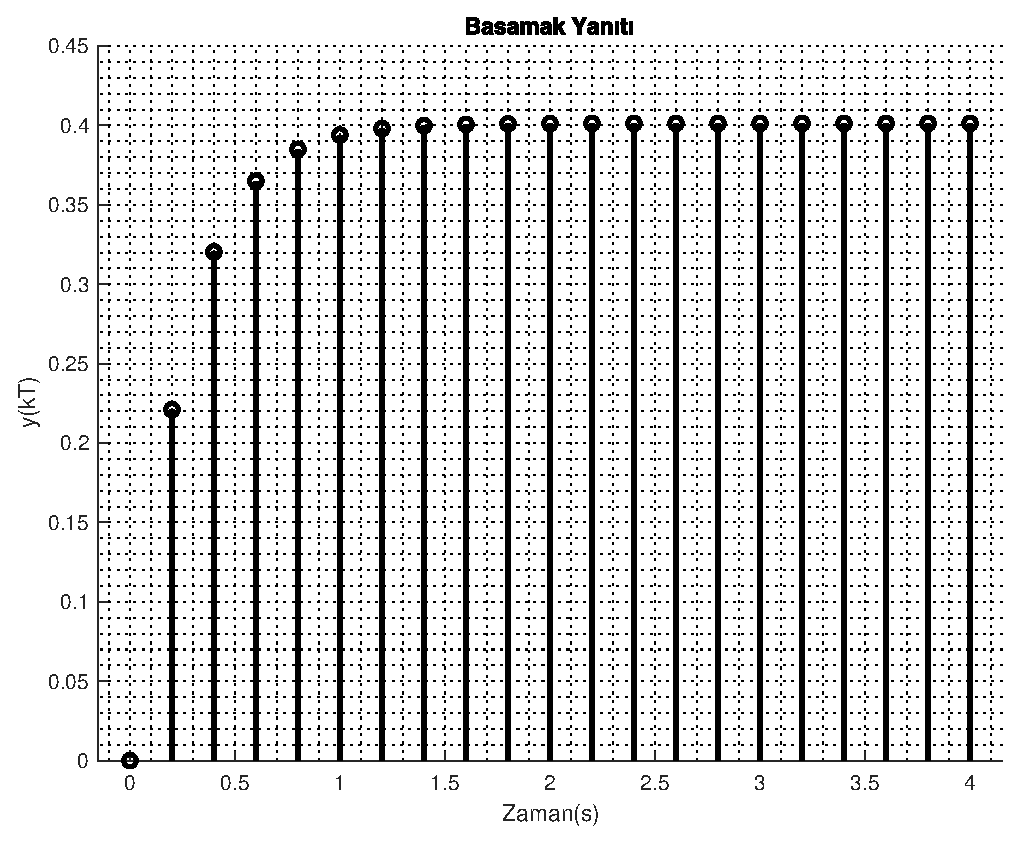
\includegraphics[width=0.75\textwidth]{img/lec7_step1}
    \caption{P kontrol için kapalı çevrim basamak yanıtı ($k=1.341$)}
    \label{fig:lec7_step1}
\end{figure}

\begin{figure}[!htb]
    \centering
    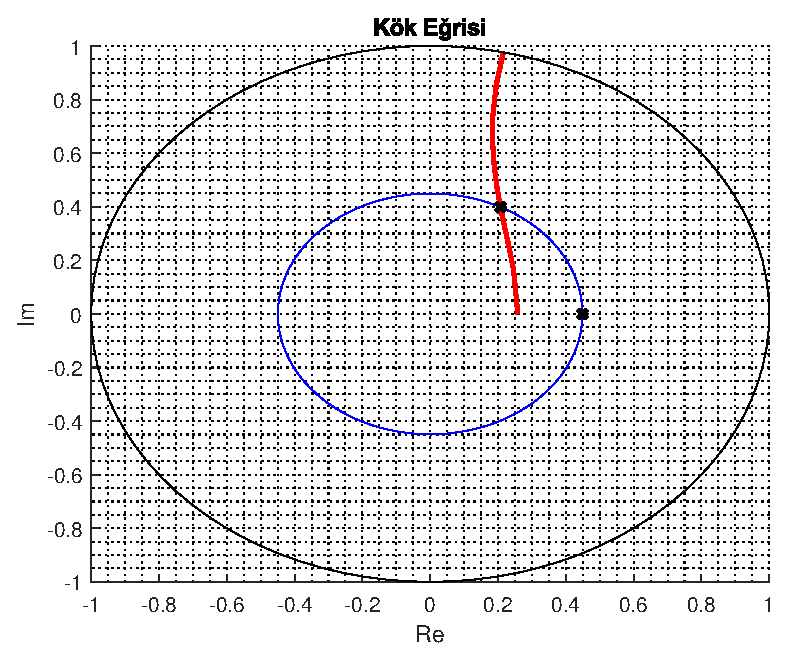
\includegraphics[width=0.75\textwidth]{img/lec7_rlocus1}
    \caption{P kontrol için kök eğrisi}
    \label{fig:lec7_rlocus1}
\end{figure}
Tasarıma ait kök eğrisi Şekil~\ref{fig:lec7_rlocus1} ile verilmiştir. Seçilen $w_n$ değerine karşılık değişken $\zeta$ değeri için eğri gösterilmiştir ve belirli bir aşıma karşılık düşen $\zeta$ değeri için tasarım noktası gösterilmiştir. Bu nokta yerleşme zamanı isteri ile elde edilen yarıçaplı çember üzerindedir. Dikkat edilirse tasarımda $\zeta$ parametresi kullanılamamıştır, çünkü kapalı çevrim karakteristik polinomunun derecesi yetersiz kalmıştır. Sadece yerleşme zamanını karşılayacak gerçel bir kutup seçilebilmektedir ve bu z tanım bölgesinde Şekil~\ref{fig:lec7_rlocus1}'deki kök eğrisinde gösterilen çembere karşılık düşmektedir. Tasarlanan P kontrolörün Kapalı çevrim transfer fonksiyonuna ait basamak yanıtı Şekil~\ref{fig:lec7_step1} ile verilmiştir. Görüldüğü üzere aşım yapmayan fakat yerleşme zamanı isterini karşılayan bir yanıt elde edilmiştir. Ayrıca, tasarım giriş sinyalini belirli bir hata ile izlemektedir.

P kontrolör için bir diğer alternatif ise 
\begin{equation}
\begin{split}
    -0.1648k+0.6703&=-0.4493\\
    k&=6.7937
\end{split}
\end{equation}
şeklindedir ve kapalı çevrim transfer fonksiyonu
\begin{equation}
    T(z)=\frac{1.1199}{z + 0.4496}
\end{equation}
şeklindedir. Basamak yanıtı Şekil~\ref{fig:lec7_step2}'de verilmiştir.

\begin{figure}[!htb]
    \centering
    \includegraphics[width=0.75\textwidth]{img/lec7_step2}
    \caption{P kontrol için kapalı çevrim basamak yanıtı($k=6.7937$)}
    \label{fig:lec7_step2}
\end{figure}

$z=-0.4496$ çözümü için s tanım bölgesine dönüşüm sonucu
\begin{equation}
\begin{split}
    z&=e^{0.2s}\\
    s&=\frac{\log{z}}{0.2}\\
    s&=5\log{(-0.4496)}\\
    s&=-3.9970 +15.7080i
\end{split}
\end{equation}
elde edilir. Sönüm oranı $\zeta$
\begin{equation}
    \begin{split}
        \theta&=\tan^{-1}\left(\frac{15.708}{3.997}\right)\\
        \theta&=75.7237^o\\
        \zeta&=\cos(\theta)\\
        \zeta&=0.2466
    \end{split}
\end{equation}
olarak hesaplanır ve aşım
\begin{equation}
        100e^{\frac{-\pi \zeta}{\sqrt{1-\zeta^2}}}=\%44.96
\end{equation}
olarak elde edilir. Birinci dereceden bir sistem s tanım bölgesinde aşım yapamazken bu durum z tanım bölgesinde geçerli değildir. Sistem kutupları s tanım bölgesinde gerçel olmak durumundadır, fakat z tanım bölgesinde bir kutup negatif gerçel olması sonucu tanım bölgesinde karmaşık sayıya karşılık düşmektedir. Bu sebeple z tanım bölgesinde aşım yapabilir. 
